\documentclass[12pt,answers]{exam}
\usepackage[margin=1in, a4paper]{geometry}

\usepackage{amsmath, amssymb, amsthm, amsbsy, amsfonts, mathtools, gensymb}
\usepackage{siunitx}

\usepackage{tikz, pgfplots}
\pgfplotsset{compat=newest}
\usepgfplotslibrary{external}
\tikzexternalize
\usepackage{graphicx}

\usepackage{setspace}
\usepackage{cancel}
\usepackage{cases}
\usepackage[nolabel, final]{showlabels}

\usepackage{microtype}
\usepackage{fourier}
\usepackage{CrimsonPro}

\usepackage[basic,italic,symbolgreek]{mathastext}
\makeatletter
\@for\@tempa:=a,b,c,d,e,h,i,k,l,m,n,o,q,r,s,t,u,v,w,x\do{%
\MTsetmathskips{\@tempa}{0.5mu}{0.5mu}}%
\makeatother
\MTsetmathskips{f}{2.5mu}{0.5mu}
\MTsetmathskips{g}{1.5mu}{0.5mu}
\MTsetmathskips{j}{2.5mu}{0.5mu}
\MTsetmathskips{p}{1.5mu}{0mu}
\MTsetmathskips{y}{1.5mu}{0.5mu}
\MTsetmathskips{z}{1mu}{0.5mu}

\newcommand{\reals}{\mathbb{R}}
\newcommand{\ints}{\mathbb{Z}}
\newcommand{\posints}{{\mathbb{Z}}^{+}}
\newcommand{\rationals}{\mathbb{Q}}
\newcommand{\complexes}{\mathbb{C}}
\renewcommand{\frac}[2]{\dfrac{#1}{#2}}
\newcommand{\oneover}[1]{\dfrac{1}{#1}}
\newcommand{\qndate}[2]{(\textbf{#1 #2})}

\pagestyle{plain}

\begin{document}
\doublespacing%
\begin{center}
  \Large
  \textbf{Problem Of The Day 2022}
\end{center}

\begin{questions}
  \question \qndate{27}{Jun} If $y$ varies inversely as $x$ and can be
  represented by the equation $y = (m-1){x}^{m^2 - 2}$, find the value of
  constant $m$.
  \begin{solution}
    \begin{align*}
      y = (m-1){x}^{m^2 - 2} & = \frac{k}{x}
      \\
      k                      & = (m-1){x}^{m^2-1}
      \\
      & = (m-1){x}^{(m+1)(m-1)} \: \left(x \neq 0\right) \\
    \end{align*}
    By definition, $y \neq 0$ as well, hence
    \begin{align*}
      (m-1){x}^{(m+1)(m-1)} & \neq 0 \\
      \therefore m          & \neq 1
    \end{align*}
  \end{solution}

  \question \qndate{28}{Jun} Which of the following is a possible plot of
  $y = x + m$ and $y = \frac{m}{x}$ on the same axes? (The graphs are not drawn
  to scale.)
  \begin{figure}[htpb]
    \centering
    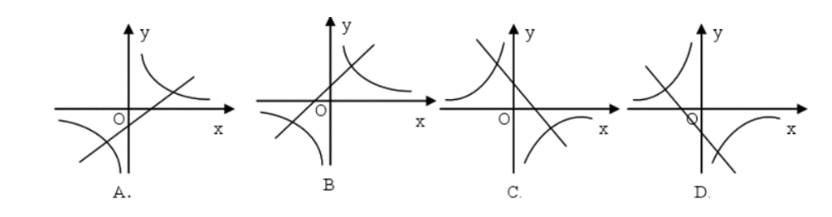
\includegraphics[scale=.8]{./images/0628_Graphs.png}
    \caption{$y = x + m$ and $y = \frac{m}{x}$.}
    \label{fig:0628_Graphs}
  \end{figure}
  \begin{solution}
    \textbf{B}.
    \begin{itemize}
      \item The straight line should be increasing, since the
        coefficient of $x$ is positive.
        \textbf{C} and \textbf{D} are eliminated.
      \item If $m > 0$, the y-intercept of the straight line could
        not be negative.
        \textbf{A} is eliminated, since the hyperbola in the same
        graph shows that $m>0$.
    \end{itemize}
  \end{solution}

  \question \qndate{29}{Jun} Given that points
  $A\left(-2,y_1\right)$, $B\left(-1,y_2\right)$,
  $C\left(1,y_3\right)$ are all on the graph of $y=-\oneover{x}$, arrange $y_1$,
  $y_2$ and $y_3$ in ascending order.
  \begin{solution}
    $y_3 < y_1 < y_2$.

    Subst. $x = -2$ into $y=-\oneover{x}$:
    \begin{align*}
      y_1 & = -\oneover{-2} \\
      & = \oneover{2}
    \end{align*}

    Subst. $x=-1$ into $y=-\oneover{x}$:
    \begin{align*}
      y_2 & = -\oneover{-1} \\
      & = 1
    \end{align*}

    Subst $x=1$ into $y=-\oneover{x}$:
    \begin{align*}
      y_3 & = -\oneover{1} \\
      & = -1
    \end{align*}
  \end{solution}

  \question \qndate{30}{Jun} Given that points
  $\left(x_1,y_1\right)$, $\left(x_2,y_2\right)$
  and $\left(x_3,y_3\right)$ are all on the graph of $y=\frac{3}{x}$, also
  $x_1<x_2<0<x_3$, arrange $y_1$, $y_2$ and $y_3$ in ascending order.
  \begin{solution}
    $y_2<y_1<y_3$.
    \begin{itemize}
      \item $y_3 > 0$ since $x_3 > 0$. Hence, $y_3$ is the greatest.
      \item $0 > x_2 > x_1$, hence $y_2 < y_1 < 0$.
    \end{itemize}
  \end{solution}

  \question \qndate{1}{Jul} Given that $y$ varies inversely as $x$ such that
  $y = \left(a-2\right){x}^{a^2-5}$, also when $x>0$, as $x$ increases, $y$
  increases. Find the equation of the hyperbola.
  \begin{solution}
    \begin{align*}
      \frac{k}{x}                                 & =
      \left(a-2\right){x}^{a^2-5}
      \\
      k                                           & =
      \left(a-2\right){x}^{a^2-4}
      \\
      & = \left(a-2\right){x}^{(a+2)(a-2)}
      \\
      \because y                                  & =
      \frac{\left(a-2\right){x}^{(a+2)(a-2)}}{x}
      \\
      \therefore \left(a-2\right){x}^{(a+2)(a-2)} & < 0
      \\
      \because a - 2 < 0                          & \text{ and }
      (a+2)(a-2) \geq 0                                                      \\
      \therefore a + 2                            & = 0
      \\
      \therefore a                                & = -2
      \\
      \therefore y                                & =
      -\frac{\left(-2-2\right)\times
      {x}^{\left(-2+2\right)\times\left(-2-2\right)}}{x} \\
      & = -\frac{4}{x}
    \end{align*}
  \end{solution}

  \question \qndate{5}{Jul} If a straight line $y = (2m - 1)x$ and a hyperbola
  $y = \frac{3-m}{x}$ has an intersection point each in Quadrant 1 and 3, what
  is the range of values of the constant $m$?
  \begin{solution}
    \begin{align*}
      \because y        & = \frac{3-m}{x} \\
      \therefore m      & < 3             \\
      \because y        & = x(2m - 1)     \\
      \therefore 2m - 1 & > 0             \\
      \therefore 0.5    & < m < 3
    \end{align*}
  \end{solution}

  \question \qndate{6}{Jul} Points $A$ and $B$ are on the hyperbola
  $y = \frac{k}{x}$. Right $\triangle AOC$
  and $\triangle BOD$ are drawn by perpendicular lines drawn from the
  two points and connecting
  the points with the origin. Compare the sizes of the areas of the
  two triangles.
  \begin{figure}[htpb]
    \centering
    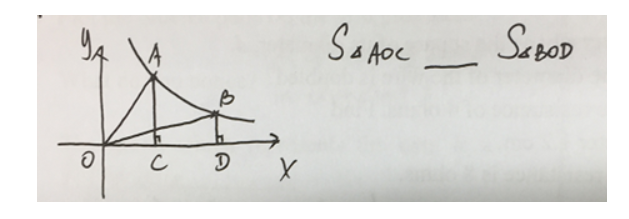
\includegraphics[scale=.8]{./images/0706_Tri.png}
    \caption{$\triangle AOC$ and $\triangle BOD$.}
    \label{fig:0706_Tri}
  \end{figure}
  \begin{solution}
    $S_{\triangle AOC} < S_{\triangle BOD}$.
    As Point $B$'s $y$-coordinate approaches 0, its $x$-coordinate
    approaches infinity,
    resulting in a triangle which approaches an infinite area. Point
    $A$ is further from
    $(\infty, 0)$ than Point $B$, so $S_{\triangle AOC} < S_{\triangle BOD}$.
  \end{solution}

  \question \qndate{7}{Jul} Points $A$ and $B$ are on the hyperbola
  $y = \frac{3}{x}$.
  Rectangles are drawn from the two points as shown. The areas
  bounded by the two
  rectangles are labelled $S_1$ and $S_2$. If the shaded area is 1
  sq. unit, find
  the sum $S_1 + S_2$.
  \begin{figure}[htpb]
    \centering
    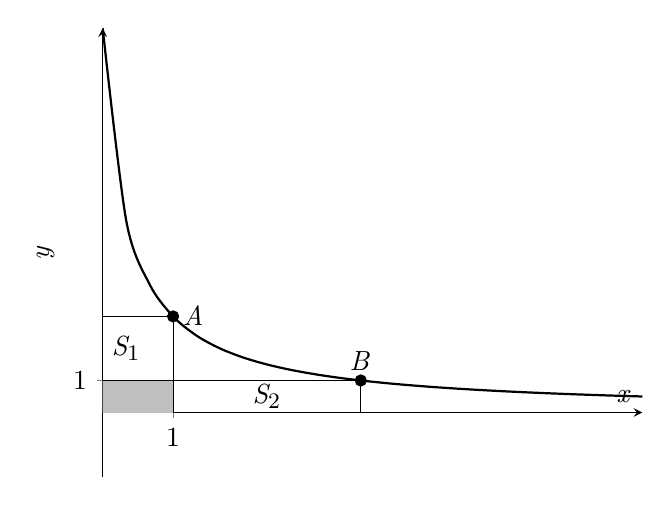
\begin{tikzpicture}
      \begin{axis}[
          domain=0:6,
          smooth,
          axis x line=center,
          axis y line=left,
          xlabel=$x$,
          ylabel=$y$,
          xtick={1},
          ytick={1},
          ymin=-2,
          scaled ticks=true,
        ]
        \addplot[black,thick] {3/x};
        \filldraw (1,3) circle[radius=2pt] node[right]{$A$};
        \filldraw (3,1) circle[radius=2pt] node[above]{$B$};
        \filldraw[lightgray] (0,0) rectangle (1,1);
        \draw (0,1) rectangle (1,3) node[pos=.5]{$S_1$};
        \draw (1,0) rectangle (3,1) node[pos=.5]{$S_2$};
      \end{axis}
    \end{tikzpicture}
    \caption{The shaded areas, $S_1$ and $S_2$.}
    \label{fig:0707_Hyper}
  \end{figure}
  \begin{solution}
    \begin{align*}
      S_1       & = \left(1 - 0\right) \times \left(\frac{3}{1}-1\right)   \\
      & = 2 \text{ sq. units}                                    \\
      S_2       & = \left(\frac{3}{3} - 0\right) \times \left(3 - 1\right) \\
      & = 2 \text{ sq. units}                                    \\
      S_1 + S_2 & = 2 + 2                                                  \\
      & = 4 \text{ sq. units}
    \end{align*}
  \end{solution}

  \question \qndate{8}{Jul} If a hyperbola $y = -\frac{3m}{x}$ and a
  straight line
  $y = kx-1$ both pass through the point $P(m,-3m)$,
  \begin{parts}
    \part find the coordinates of $P$ and the equations of the
    hyperbola and the straight line.
    \begin{solution}
      \begin{align*}
        y & = -\frac{3m}{x}\label{eq:0708a}\tag{1} \\
        y & = kx - 1\label{eq:0708b}\tag{2}
      \end{align*}
      Subst. $x = m$, $y = -3m$ into \eqref{eq:0708a}:
      \begin{align*}
        -3m             & = -\frac{3m}{m}            \\
        \therefore m    & = 1                        \\
        \therefore P(1, & -3)\label{eq:0708c}\tag{3}
      \end{align*}
      We can substitute the values obtained in \eqref{eq:0708c} into
      \eqref{eq:0708b}:
      \begin{align*}
        -3           & = k - 1 \\
        \therefore k & = -2
      \end{align*}

      The equations of the hyperbola and the straight line, are, thus:
      \begin{align*}
        y & = -\frac{3}{x} \\
        y & = -2x - 1
      \end{align*}
    \end{solution}

    \part If the points $M(a,y_1)$ and $N(a+1,y_2)$ are both on the
    straight line,
    explain clearly why $y_1>y_2$.
    \begin{solution}
      Substitute the $x$- and $y$-coordinates of both points into the
      equation of the line.
      \begin{align*}
        y_1              & = -2a - 1                              \\
        y_2              & = -2(a+1) - 1                          \\
        & = -2a - 3                              \\
        \because -2a - 1 & > -2a - 3 \text{, where } a \in \reals \\
        \therefore y_1   & > y_2
      \end{align*}
    \end{solution}
  \end{parts}

  \question \qndate{12}{Jul} The line $y = x$ meets the hyperbola
  $y=\oneover{x}$
  at points $A$ and $C$. Vertical lines from $A$ and $C$ meet the
  $x$-axis at points $B$
  and $D$ respectively. Find the area of the quadrilateral $ABCD$.
  (The diagram is
  not drawn to scale.)
  \begin{figure}[htpb]
    \centering
    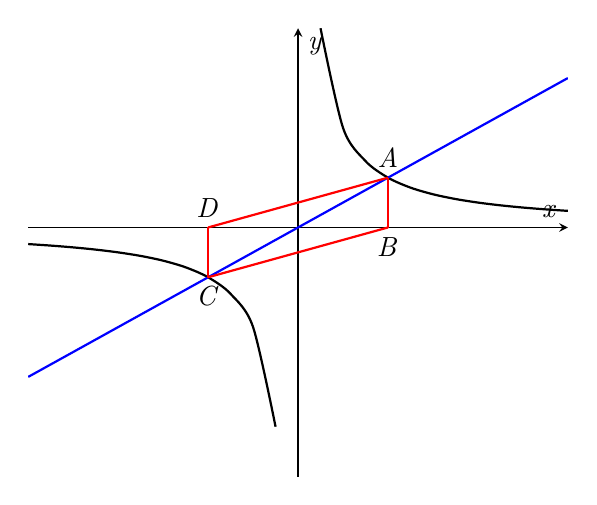
\begin{tikzpicture}
      \begin{axis}[
          axis x line=middle,
          axis y line=middle,
          xlabel=$x$,
          ylabel=$y$,
          domain=-3:3,
          ticks=none,
          ymin=-5,
          smooth,
          unbounded coords=jump,
        ]
        \addplot[black,thick,mark=none]  {1/x};
        \addplot[blue,thick]  expression {x};
        \addplot[mark=none] coordinates {(1,1)} node[above]{$A$};
        \addplot[mark=none] coordinates {(-1,-1)} node[below]{$C$};
        \addplot[mark=none,red,thick] coordinates {(1,1)(1,0)};
        \addplot[mark=none,red,thick] coordinates {(-1,-1)(-1,0)};
        \addplot[mark=none] coordinates {(-1,0)} node[above]{$D$};
        \addplot[mark=none] coordinates {(1,0)} node[below]{$B$};
        \addplot[mark=none,red,thick] coordinates {(-1,0)(1,1)};
        \addplot[mark=none,red,thick] coordinates {(1,0)(-1,-1)};
      \end{axis}
    \end{tikzpicture}
    \caption{Quadrilateral $ABCD$.}
    \label{fig:0712}
  \end{figure}
  \begin{solution}
    \begin{align*}
      x                 & = \oneover{x}                               \\
      \therefore x      & = \pm 1                                     \\
      \therefore A(1,1) & \text{ and } C(-1,-1)                       \\
      S_{ABCD}          & = 1 \times \left[1 - \left(-1\right)\right] \\
      & = 2 \text{ sq. units}
    \end{align*}
  \end{solution}

  \question \qndate{13}{Jul} A ladder $AB$ of length \qty{2.5}{\metre} has its
  foot $B$ \qty{1.5}{\metre} away from a wall. The ladder is then moved to a new
  position $ED$. The foot of the ladder is moved \qty{.5}{\metre} from the
  original position $B$. Find the distance the top of the ladder drops,
  the length of $AE$.

  \begin{figure}[htpb]
    \centering
    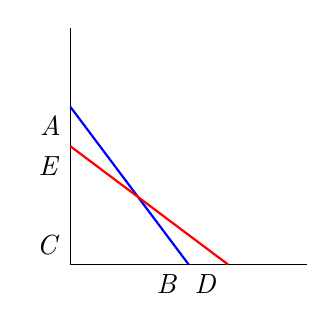
\begin{tikzpicture}
      \draw[black,thin]  (0,0)--(0,3);
      \node[mark=none,anchor=south east] (C) at (0,0) {$C$};
      \draw[black,thin]  (0,0)--(3,0);
      \draw[blue,thick] (1.5,0)--(0,2);
      \node[mark=none,anchor=north east] (A) at (0,2) {$A$};
      \node[mark=none,anchor=north east] (B) at (1.5,0) {$B$};
      \draw[red,thick] (2,0)--(0,1.5);
      \node[mark=none,anchor=north east] (E) at (0,1.5) {$E$};
      \node[mark=none,anchor=north east] (D) at (2,0) {$D$};
    \end{tikzpicture}
    \label{fig:Ladder}
    \caption{The ladder, before and after.}
  \end{figure}

  \begin{solution}
    \begin{align*}
      AC                     & = \sqrt{{2.5}^2 - {1.5}^2}                    \\
      & = \qty{2}{\metre}                             \\
      EC                     & = \sqrt{{2.5}^2 - {\left(1.5 + 0.5\right)}^2} \\
      & = \qty{1.5}{\metre}                           \\
      \text{height dropped } & = 2 - 1.5                                     \\
      & = \qty{0.5}{\metre}
    \end{align*}
  \end{solution}

  \question \qndate{14}{Jul} In $\triangle ABC$, $\angle B = \ang{22.5}$. The
  perpendicular bisector of $AB$ intersects $BC$ at point $D$ and ${BD}^2 = 72$.
  $AE \perp BC$. Find $AE$.
  \begin{figure}[htpb]
    \centering
    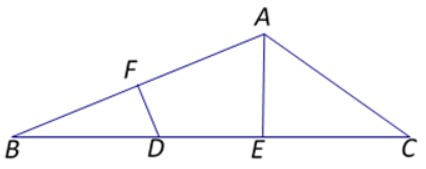
\includegraphics[scale=0.5]{./images/0714_Tri.jpeg}
    \caption{Triangle $\triangle ABC$.}
    \label{fig:0714_Tri}
  \end{figure}

  \begin{solution}
    \begin{align*}
      \angle FAD            & = \angle B                       \\
      & = \ang{22.5}                     \\
      BD                    & = AD                             \\
      & = \sqrt{72}                      \\
      \angle FDA            & = 90 - 22.5                      \\
      & = \ang{67.5}                     \\
      \angle FDB            & = \angle FDA = \ang{67.5}        \\
      \therefore \angle ADE & = 180 - 67.5 \times 2            \\
      & = \ang{45}                       \\
      \sin \angle ADE       & = \frac{AE}{\sqrt{72}}           \\
      AE                    & = \sqrt{72} \times \sin \ang{45} \\
      & = \frac{\sqrt{72}}{\sqrt{2}}     \\
      & = 6
    \end{align*}
  \end{solution}

  \question \qndate{15}{Jul} In $\triangle ABC$, $\angle A =
  \ang{90}$. The point
  $P$ is the midpoint of $AC$. $PD \perp BC$, $BC = 9$ and $DC = 3$.
  Find $AB$.
  \begin{figure}[htpb]
    \centering
    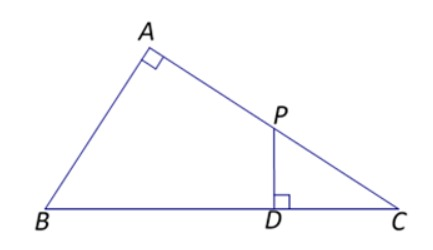
\includegraphics[scale=.5]{images/0715_Tri.jpeg}
    \caption{Triangle $\triangle ABC$.}
    \label{fig:0715_Tri}
  \end{figure}
  \begin{solution}
    \begin{align*}
      \sqrt{3^2 + {PD}^2} & = \sqrt{6^2 + {PD}^2 - {AB}^2} \\
      {PD}^2 + 9          & = {PD}^2 + 36 - {AB}^2         \\
      27 - {AB}^2         & = 0                            \\
      \therefore AB       & = \sqrt{27}
    \end{align*}
  \end{solution}

  \question \qndate{18}{Jul} In $\triangle ABC$, $AB=7$, $BC=6$, $AC=4$, and
  $AD$ and $AE$ are the height and the median on the side $BC$, such
  that $BE=EC$
  and $AD\perp BC$. Find the length of $DE$.
  \begin{figure}[htpb]
    \centering
    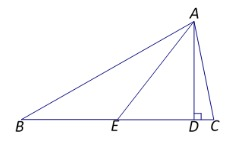
\includegraphics[scale=.7]{images/0718_Tri.jpeg}
    \label{fig:0718_Tri}
    \caption{$\triangle ABC$.}
  \end{figure}
  \begin{solution}
    \begin{align*}
      3^2 + {DE}^2 & = 7^2       \\
      {DE}^2       & = 7^2 - 3^2 \\
      & = 40        \\
      {DE}         & = \sqrt{40}
    \end{align*}
  \end{solution}

  \question \qndate{19}{Jul} The lengths of three sides of a triangle
  are $m^2-n^2$,
  $m^2+n^2$ and $2mn$, where $m$ and $n$ are positive integers and
  $m>n$. Determine
  if this triangle is a right triangle or not. Show your reason clearly.
  \begin{solution}
    Yes. Assuming that the triangle \textbf{is} a right triangle,
    $m^2+n^2$ would be the hypotenuse.
    \begin{align*}
      {\left(2mn\right)}^2 + {\left(m^2 - n^2\right)}^2 & =
      {\left(m^2+n^2\right)}^2                    \\
      4m^2n^2 + m^4 - 2m^2n^2 + n^4                     & = m^4 +
      2m^2n^2 + n^4 \text{ (true, proven.)}
    \end{align*}
  \end{solution}

  \question \qndate{20}{Jul} The lengths of the three sides of a
  triangle satisfy
  $a^2c^2 - b^2c^2 = a^4-b^4$. Determine the type of triangle it is.
  Show your reason
  clearly.
  \begin{solution}
    It is a right triangle.
    \begin{align*}
      a^2c^2 - b^2c^2                     & = a^4-b^4
      \\
      c^2\left(a-b\right)\left(a+b\right) & =
      \left(a^2+b^2\right)\left(a-b\right)\left(a+b\right) \\
      c^2                                 & = a^2 + b^2
    \end{align*}
  \end{solution}

  \question \qndate{21}{Jul} A corner of a rectangle $ABCD$ is folded
  along the line $AE$,
  such that the vertex $D$ lands exactly on the opposite side $BC$ at point $F$.
  If $AB=8$ and $BC=10$, find the length of $EC$.
  \begin{figure}[htpb]
    \centering
    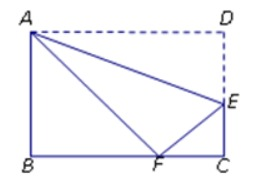
\includegraphics[scale=.6]{images/0721_Tri.jpeg}
    \caption{Rectangle $ABCD$.}
    \label{fig:0721_Tri}
  \end{figure}
  \begin{solution}
    \begin{align*}
      BC = AD                  & = AF = 10                               \\
      BF                       & = \sqrt{{10}^2-8^2}                     \\
      & = 6                                     \\
      \therefore FC            & = 10 - 6                                \\
      & = 4                                     \\
      \angle BAF               & = \angle EFC \text{ (alt. ext. angles)} \\
      \angle ECF               & = \angle ABF \text{ (given)}            \\
      \therefore \triangle ABF & \simeq \triangle FCE \text{ (AA)}       \\
      \therefore \frac{EC}{AB} & = \frac{CF}{BF}                         \\
      \frac{EC}{8}             & = \frac{4}{6}                           \\
      \therefore EC            & = \frac{16}{3}
    \end{align*}
  \end{solution}

  \question \qndate{22}{Jul} In an isosceles $\triangle ABC$, $AB=AC$. $P$ is a
  random point on $BC$. Show that ${AB}^2 - {AP}^2 = PB \times PC$.
  \begin{figure}[htpb]
    \centering
    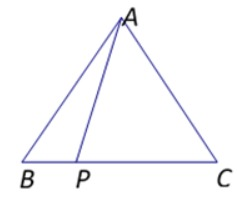
\includegraphics[scale=.6]{images/0722_Tri.jpeg}
    \caption{Isosceles $\triangle ABC$.}
    \label{fig:0722_Tri}
  \end{figure}
  \begin{solution}
    We can construct a line $AO \perp BC$, thereby bisecting $BC$.
    \begin{align*}
      AB^2 - AP^2 & = AO^2 + OB^2 - \left(AO^2 + PO^2\right) \\
      & = OB^2 - PO^2                            \\
      & = (OB+PO)(OB-PO)                         \\
      & = PC \times PB                           \\
      & = PB \times PC
    \end{align*}
  \end{solution}

  \question \qndate{25}{Jul} In $\triangle ABC$, $\angle A =
  \ang{30}$ and $\angle B = \ang{45}$.
  Points $D$ and $E$ are on sides $AB$ and $AC$ respectively, such
  that $AE=ED=EC$.
  Find the ratio $\frac{AD^2}{BC^2}$.
  \begin{figure}[htpb]
    \centering
    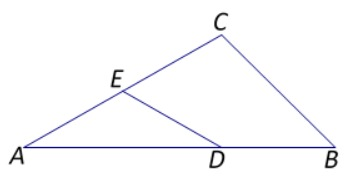
\includegraphics[scale=.6]{images/0725_Tri.jpeg}
    \caption{$\triangle ABC$.}
    \label{fig:0725_Tri}
  \end{figure}

  \question \qndate{26}{Jul} In $\triangle ABC$, $a$, $b$ and $c$ are
  the three sides.
  $\angle C = \ang{90}$, $\angle A = \ang{60}$, $a + b = 3 +
  \sqrt{3}$. Find $a$, $b$
  and $c$.
  \begin{solution}
    By using trigonometric ratios,
    \begin{align*}
      AB : AC : BC & = 2 : 1 : \sqrt{3}
    \end{align*}
    Multiply the ratio by $\sqrt{3}$:
    \begin{align*}
      AB : AC : BC       & = 2\sqrt{3} : \sqrt{3} : 3 \\
      \because a + b     & = 3 + \sqrt{3}             \\
      \therefore BC + AC & = a + b                    \\
      \therefore c       & = AB = 2\sqrt{3}           \\
    \end{align*}
    However, we cannot determine $a$ and $b$ because of the
    commutative law of addition.
    \begin{align*}
      \begin{cases}
        a & = 3 \text{ if } b = \sqrt{3} \text{ else } \sqrt{3} \\
        b & = 3 \text{ if } a = \sqrt{3} \text{ else } \sqrt{3} \\
        c & = 2\sqrt{3}
      \end{cases}
    \end{align*}
  \end{solution}

  \question \qndate{27}{Jul} In $\triangle ABC$, $\angle ACB =
  \ang{90}$, $AB \perp CD$,
  $AC = \sqrt{5}$, $BC = 2$. Find $\sin\angle ACD$.
  \begin{figure}[htpb]
    \centering
    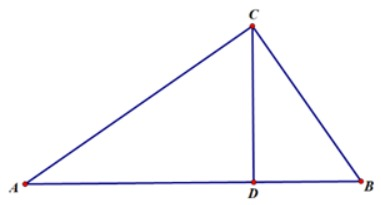
\includegraphics[scale=.5]{images/0727_Tri.jpeg}
    \caption{$\triangle ABC$.}
    \label{fig:0727_Tri}
  \end{figure}
  \begin{solution}
    \begin{align*}
      \angle CAB                & = \arctan \frac{2\sqrt{5}}{5}
      \\
      \angle ACD                & = \left(90-\arctan
      \frac{2\sqrt{5}}{5}\right) \degree \\
      \therefore \sin\angle ACD & = \sin \left(90-\arctan
      \frac{2\sqrt{5}}{5}\right)    \\
      & = \frac{2}{3}
    \end{align*}
  \end{solution}

  \question \qndate{28}{Jul} For acute angle $\alpha$, fill in the blanks
  with $>$, $=$, or $<$.
  \begin{solution}
    \begin{align*}
      \begin{cases}
        \because \alpha = \ang{45} &\therefore \sin \alpha = \cos \alpha \\
        \because \alpha < \ang{45} &\therefore \sin \alpha < \cos \alpha \\
        \because \alpha > \ang{45} &\therefore \sin \alpha > \cos \alpha \\
      \end{cases}
    \end{align*}
  \end{solution}

  % \question \qndate{29}{Jul} In $\triangle ABC$, $\angle
  % ACB=\ang{90}$, $CD\perp AB$,
  % and $AC>BC$. Which of the following ratios of sides is not equal
  % to the value of
\end{questions}
\end{document}
